% hm-05-science.tex

\documentclass[xcolor=dvipsnames]{beamer}

\usepackage{graphicx}
% \usepackage{wrapfig}
% \usepackage{colortbl}
\usepackage{alltt}
% \definecolor{myblue}{rgb}{0.8,0.85,1}

\mode<presentation>
{
  \usetheme{Warsaw}
  \setbeamercovered{transparent}
}
% \usecolortheme[named=OliveGreen]{structure}
\setbeamertemplate{navigation symbols}{} 
\setbeamertemplate{blocks}[rounded][shadow=true] 

\newif\ifBCITCourse
\BCITCoursetrue
\BCITCoursefalse
\newif\ifWhichCourse
\WhichCoursetrue
% \WhichCoursefalse
\ifBCITCourse
\ifWhichCourse
\newcommand{\CourseName}{Statistics for Food Technology}
\newcommand{\CourseNumber}{MATH 1441}
\newcommand{\CourseInst}{BCIT}
\else
\newcommand{\CourseName}{Calculus for Geomatics}
\newcommand{\CourseNumber}{MATH 1511}
\newcommand{\CourseInst}{BCIT}
\fi
\else
\newcommand{\CourseName}{Philosophy and Literature}
\newcommand{\CourseNumber}{PHIL 375}
\newcommand{\CourseInst}{UBC}
\fi

\title{Science and Interpretation}
\subtitle{{\CourseNumber}, {\CourseInst}}

\author{\CourseName}

\date{October 26, 2017}

\begin{document}

\begin{frame}
  \titlepage
\end{frame}

\begin{frame}
  \frametitle{iClicker Question}
Choose from the following options. This item will be graded.
\begin{block}{iClicker Question}
Which of these principles is Carnap's?
\end{block}
\begin{description}
\item[A\hspace{.2in}$\blacktriangleright$] the principle of contiguity
\item[B\hspace{.2in}$\blacktriangleright$] the principle of reciprocity
\item[C\hspace{.2in}$\blacktriangleright$] the principle of equivalence
\item[D\hspace{.2in}$\blacktriangleright$] the principle of tolerance
\end{description}
\end{frame}

\begin{frame}
  \frametitle{iClicker Question}
Choose from the following options. This item will be graded.
\begin{block}{iClicker Question}
Einstein and Perrin's work on Brownian motion scientifically
established 
\end{block}
\begin{description}
\item[A\hspace{.2in}$\blacktriangleright$] the existence of galaxies
\item[B\hspace{.2in}$\blacktriangleright$] the existence of space curvature
\item[C\hspace{.2in}$\blacktriangleright$] the existence of atoms
\item[D\hspace{.2in}$\blacktriangleright$] the existence of gravitational waves
\end{description}
\end{frame}

\begin{frame}
  \frametitle{iClicker Question}
Choose from the following options. This item will be graded.
\begin{block}{iClicker Question}
How, according to Popper, should we test a theory?
\end{block}
\begin{description}
\item[A\hspace{.2in}$\blacktriangleright$] by induction
\item[B\hspace{.2in}$\blacktriangleright$] by abduction
\item[C\hspace{.2in}$\blacktriangleright$] by deduction
\item[D\hspace{.2in}$\blacktriangleright$] by obduction
\end{description}
\end{frame}

\begin{frame}
  \frametitle{iClicker Question}
Choose from the following options. This item will be graded.
\begin{block}{iClicker Question}
What distinguishes, according to Popper, a scientific problem from a
non-scientific problem?
\end{block}
\begin{description}
\item[A\hspace{.2in}$\blacktriangleright$] the scientific problem can
  be answered one way or another by a proof
\item[B\hspace{.2in}$\blacktriangleright$] the scientific problem is
  stated such that there is a method for verification
\item[C\hspace{.2in}$\blacktriangleright$] the scientific problem is
  stated to make it possible for a hypothesis to be falsified
\item[D\hspace{.2in}$\blacktriangleright$] the scientific problem can
  be solved a priori, without reference to experience
\end{description}
\end{frame}

\begin{frame}
  \frametitle{Sherlock Holmes}
  \begin{quote}
    Holmes walks into the old second hand store and looks across the
    counter. The man standing there glances up before returning to his
    bookkeeping. Holmes turns to his companion and says, ``That, my
    dear Watson, is the man we are looking for.'' ``But Holmes, how on
    Earth can you know such a thing? You've not even spoken to him!''
    ``Ah, but you see Watson, it is simple. I noticed that his beard is
    ragged and untrimmed, but its style implies that it is usually
    well kept. This means that he had little or no time this morning
    to undertake his usual particulars. He is wheezing slightly,
    showing that he was out of the shop this morning in the dense smog
    we have been having all over London. And, of course, he is wearing
    the stolen watch on a chain in his waistcoat.'' ``Eee Gads Holmes, I
    just don't know how you do it!'', exclaims Watson.
  \end{quote}
\end{frame}

\begin{frame}
  \frametitle{Inductive Deductive Abductive}
  \begin{figure}[h]
    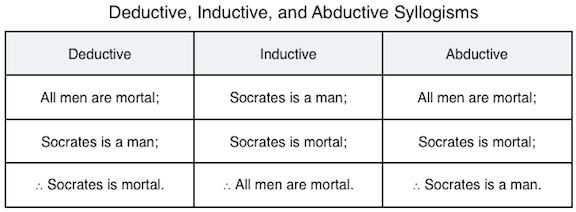
\includegraphics[scale=0.55]{./inabde.png}
  \end{figure}
\end{frame}

\begin{frame}
  \frametitle{Charlie Brown I}
  \begin{figure}[h]
    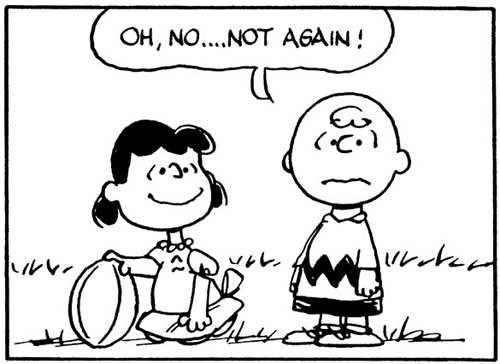
\includegraphics[scale=0.5]{./charliebrown1.jpg}
  \end{figure}
\end{frame}

\begin{frame}
  \frametitle{Charlie Brown II}
  \begin{figure}[h]
    
\includegraphics[scale=0.5]{./charliebrown2.png}
  \end{figure}
\end{frame}

\begin{frame}
  \frametitle{The Problem of Induction}
  You see many white swans. What is your justification for believing
  that all swans are white? You may say, ``I've used induction all my
  life, and it has worked really well---after seeing many white swans,
  the next swan was always white, so induction is predictive!''
  However, your reasoning is circular. You have used inductive
  reasoning to justify inductive reasoning.
\end{frame}

\begin{frame}
  \frametitle{The Problem of Induction}
Karl Popper expresses this objection as follows: if in science we use
inductive reasoning (as Hans Reichenbach claims), then there must be
such a thing as an inductive principle. This principle cannot be a
logical truth, for it is logically possible that induction fails.
\begin{block}{Bertrand Russell, ``On Induction''}
  The man who has fed the chicken every day throughout its life at
  last wrings its neck instead, showing that more refined views as to
  the uniformity of nature would have been useful to the chicken.
\end{block}
Something which is true not by logic alone is sometimes called a
synthetic truth. Logic does not disallow the possibility of its
negation being true. Propositions (the kind of thing that can be true
or false) are therefore necessarily true (necessary), contingently
true or false (possible), or necessarily false (impossible), although
you need to be careful with these attributions (men and U.S.
presidents).
\end{frame}

\begin{frame}
  \frametitle{The Problem of Induction}
  If the principle of induction is both a general law and a synthetic
  truth, the only way to justify it is by induction! Therefore, if
  induction is at the heart of science, science is in danger of
  cardiac arrest. Popper's solution: ditch induction. Science is based
  on deductive reasoning. (Kant had a similarly ingenious solution for
  this problem: the synthetic \emph{a priori}; but Kant was famously
  wrong about some things that he thought were synthetic a priori
  truths, such as that space is Euclidean. A proposition is true a
  priori if you can know that it is true without reference to
  experience.)
\end{frame}

\begin{frame}
  \frametitle{Scientific Method}
  Just as Mill did for ethics, Popper formulates a two-step procedure
  for science based on art (the creation of hypotheses) and
  experiment. The first step has echoes of the hermeneutic method in
  it: there is an ``irrational element'' and ``creative intuition''
  (Henri Bergson). A scientific theory is first formulated ``by
  intuition, based upon something like an intellectual love
  (Einf{\"u}hlung) of the objects of experience'' (32).
\end{frame}

\begin{frame}
  \frametitle{Four Tests of a Scientific Hypothesis}
  \begin{enumerate}
  \item test the internal logical consistency of the system
  \item test the character of the hypothesis---is it empirical or
    tautological?
  \item test how the hypothesis stacks up against already existing
    scientific theories---is it stronger or weaker or inconsistent
    with them?
  \item test deductive implications (modus tollens) (32f)
  \end{enumerate}
Testing does not confirm a theory or make it more probable. It only
corroborates it. Both Relativity Theory and Quantum Mechanics are
extremely well-corroborated, but mutually incompatible in their
present version. GRT, for example, was yet again corroborated last
year by the discovery of gravitational waves.
\end{frame}

\begin{frame}
  \frametitle{Examples}
  \begin{itemize}
  \item Steady State theory vs Big Bang theory
    \begin{description}
    \item[radio waves] bright radio sources are found more numerously
      in far-away galaxies
    \item[CMB] before the universe broke up into chunks (stars and
      galaxies), it emitted radiation that can still be measured as
      cosmic microwave background
    \end{description}
  \end{itemize}
\end{frame}

\begin{frame}
  \frametitle{The Problem of Demarcation}
Hume's problem and Kant's problem. How do we distinguish between
scientific questions and metaphysical speculation? The problem with
positivism (verificationism) is that it pours out the baby with the
bathwater. Universal statements about nature are as nonsensical and
meaningless as Hume's ``metaphysical twaddle'' because positivists
fail to give rules for how they might be established empirically
(the problem of induction).

\bigskip 

Poppers solution: \alert{falsifiability} as a criterion of
demarcations. 
\end{frame}

\begin{frame}
  \frametitle{Unrepeatable, Unique Events}
  When Popper talks about science, his favourite example is always
  theoretical physics with its universal laws. Many theories in
  science are about singular statements: climate change, evolution,
  extra-terrestrial life, expanding universe.
  \begin{block}{Karl Popper}
    Any controversy over the question whether events which are in
    principle unrepeatable and unique ever do occur cannot be decided
    by science: it would be a metaphysical controversy. (46)
  \end{block}
Here is an example of a prediction by evolutionary theory (although,
if it were experimentally falsified, it wouldn't falsify evolutionary
theory): high-ranking mothers should give more parental care to sons;
low-ranking mothers to daughters. 
\end{frame}

\begin{frame}
  \frametitle{The Role of Tradition}
  I have friends who claim that they have never experienced a
  supernatural phenomenon, but that they know and trust other people
  who have told them about experiencing a supernatural phenomenon.
  Popper's verdict is clear:
  \begin{quote}
    Can any statement be justified by the fact that K.R.P. is utterly
    convinced of its truth? The answer is no. (46)
  \end{quote}
  One problem that Popper faces is that falsifications are also
  subjectively experienced unique events. ``There can be no ultimate
  statements in science: there can be no statements in science which
  cannot be tested'' (47). Statements of higher levels of
  universality are tested by statements of lower levels of
  universality, ad infinitum. 
\end{frame}

\begin{frame}
  \frametitle{The Ad-Hoc Auxiliary Hypothesis Problem}
  \begin{equation}
    \label{eq:uangaiso}
\begin{array}{l}
  A\supset{}C \\
  \urcorner{}C \\ \hline
  \therefore{}\urcorner{}A
\end{array}
\mbox{ is valid but }
\begin{array}{l}
  A\wedge{}B\supset{}C \\
  \urcorner{}C \\ \hline
  \therefore{}\urcorner{}A
\end{array}
\mbox{ is not.}\notag
  \end{equation}

\bigskip

Falsification fails if you can introduce an auxiliary
hypothesis (Duhem-Quine problem: it is impossible to test a scientific
theory in isolation). Popper's solution: a scientist is not trying to
keep a theory alive. Popper favours a view of science in which only
the fittest theories survive. 
\end{frame}

\begin{frame}
  \frametitle{Ill-Posed Questions}
  \begin{block}{Immanuel Kant: Critique of Pure Reason}
    For if the question is absurd in itself and demands unnecessary
    answers, then, besides the embarrassment of the one who proposes
    it, it also has the disadvantage of misleading the incautious
    listener into absurd answers, and presenting the ridiculous sight
    (as the ancients said) of one person milking a billy-goat while
    the other holds a sieve underneath.
  \end{block}
\end{frame}

\begin{frame}
  \frametitle{Ill-Posed Questions}
  \begin{block}{Rudolf Carnap: Intellectual Autobiography}
    Most of the controversies in traditional metaphysics appeared to
    me sterile and useless. When I compared this kind of argumentation
    with investigations and discussions in empirical science or in the
    logical analysis of language, I was often struck by the vagueness
    of the concepts used and by the inconclusive nature of the
    arguments. I was depressed by disputations in which the opponents
    talked at cross purposes; there seemed hardly any chance of mutual
    understanding, let alone of agreement, because there was not even
    a common criterion for deciding the controversy.
\end{block}
\end{frame}

\begin{frame}
  \frametitle{Ill-Posed Questions}
  \begin{block}{Rudolf Carnap: Intellectual Autobiography}
    Many theses of traditional metaphysics are not only useless, but
    even devoid of cognitive content. They are pseudo-sentences, that
    is to say, they seem to make assertions because they have the
    grammatical form of declarative sentences, and the words
    occurring in them have many strong and emotionally loaded
    associations, while in fact they do not make any assertions, do
    not express any propositions, and are therefore neither true nor
    false.
\end{block}
\end{frame}

\begin{frame}
  \frametitle{First Philosophy}
  \begin{figure}[h]
    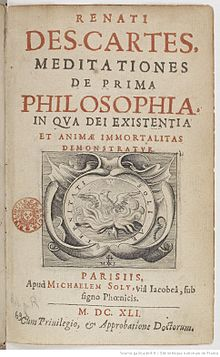
\includegraphics[scale=0.5]{./prima.jpg}
  \end{figure}
  \emph{Meditations on First Philosophy} (subtitled \emph{In Which the
    Existence of God and the Immortality of the Soul Are
    Demonstrated}) is a treatise by Ren{\'e} Descartes
  first published in 1641 (in Latin).
\end{frame}

\begin{frame}
  \frametitle{Rational Reconstruction}
  \alert{Rational reconstruction} refers to the way Rudolf Carnap (a
  logical positivist) was trying to solve the problem of demarcation.
  According to Carnap, a sentence needs to be part of a linguistic
  framework. Here are some examples:
  \begin{itemize}
  \item ``five plus seven is twelve'' is a sentence in the linguistic
    framework of mathematics, its truth follows from the rules of the
    linguistic framework
  \item ``I have hands'' is a sentence in the linguistic framework of
    observable things such as tables, chairs, bodies, etc.
  \item ``The positron is the antimatter counterpart of the electron''
    is a sentence in the linguistic framework of unobservables in
    theoretical physics (Dirac predicted its existence using
    mathematics, Carl David Anderson took a cloud chamber picture of
    its trail in 1932)
  \end{itemize}
\end{frame}

\begin{frame}
  \frametitle{Rational Reconstruction}
The truth and falsity of a sentence can only be evaluated within a
linguistic framework, thus the meaningless of the skeptic's quest to
show that ``I have hands'' cannot be justified. Linguistic frameworks
need clear rules about verification, thus statements such as ``the
church is the bride of Christ'' are problematic (and with it all of
hermeneutics?).

\bigskip

Since what it is to be real is to be an element of the linguistic
framework, it makes no sense to ask the question whether the
linguistic framework is real. However, it is permitted to ask the
\emph{pragmatic} question how effective, simple, fruitful, efficient,
and conducive to the aim for which the language is intended the
linguistic framework is (Penelope Maddy, 70).
\end{frame}

\begin{frame}
  \frametitle{Principle of Tolerance}
  \begin{block}{Rudolf Carnap: The Logical Syntax of Language}
    It is not our business to set up prohibitions, but to arrive at
    conventions. In logic, there are no morals. Everyone is at
    liberty to build her own logic, i.e.\ her own form of language, as
    she wishes. All that is required of her is that, if she wishes to
    discuss it, she must state her methods clearly and give
    syntactical rules instead of philosophical arguments.
  \end{block}
\end{frame}

\begin{frame}[fragile]
  \frametitle{Brownian Motion}
The French chemist Joseph Louis Proust noticed at the end of the 18th
century that two tin oxides (known today as tin monoxide and tin
dioxide) would split up into tin and oxygen at the following ratios:

\medskip

\begin{center}
\begin{tabular}{|l|r|r|}\hline
  & tin & oxygen \\ \hline
  tin oxide I & 88.1\% & 11.9\% \\ \hline
  tin oxide II & 78.7\% & 21.3\% \\ \hline
\end{tabular}
\end{center}

\medskip

This means that if you were to reconstitute the tin oxides, you would
use 100 grams of tin and 13.5 grams of oxygen or 27 grams of oxygen
respectively. The ratio of the oxygen for the different tin oxides is
1:2. Chemists found these small ratios at some regularity and began to
wonder if they were representative of the atomic structure of matter
(abduction).
\end{frame}

\begin{frame}
  \frametitle{Brownian Motion}
  An Italian scientist, Amedeo Avogadro, proposed in 1811 that no
  matter how heavy a gas is, at constant temperature, volume, and
  pressure it comprised the same number of molecules. Indeed, when you
  mix two litres of hydrogen with one litre of oxygen you get two
  litres of water vapour.

  \bigskip

  If we were to use this as proof for the
  atomic structure of matter, it would be circular, because Avogadro's
  Law presupposes the atomic structure of matter. Abductively
  speaking, however, the atomic structure of matter hypothesis makes
  sense of the data, while the alternative fluid structure of matter
  hypothesis lacks an explanation.
\end{frame}

\begin{frame}
  \frametitle{Brownian Motion}
  Albert Einstein, a German physicist, used Brownian motion to deliver
  the final piece of discriminating evidence in favour of
  atoms/molecules. Here is an illustration of Brownian motion:
  \begin{alltt}
    \tiny https://upload.wikimedia.org/wikipedia/commons/c/c2/Brownian\_motion\_large.gif
  \end{alltt}
  Einstein modeled Brownian motion using differential equations. Jean
  Perrin, a French physicist, conducted experiments that confirmed
  Einstein's results (the equations successfully predicted the
  observations). Even though no one has ever perceived an atom,
  Einstein and Perrin's work is as close to a scientific proof of the
  existence of atoms as you will get.
\end{frame}

\begin{frame}
  \frametitle{Brownian Motion}
  \begin{description}
  \item[Rudolf Carnap] Atoms do not exist in the linguistic framework
    for ``things'' (medium-sized objects that humans can perceive; J.L.
    Austin called them ``middle-sized dry goods''). They only exist in
    the linguistic framework of particle physics.
  \end{description}
  Carnap's clash with Einstein was more over the nature of space than
  over the existence of atoms. Carnap thought that despite the
  overwhelming evidence in favour of the gravitational curvature of
  space (see Eddington's 1919 experiment), ultimately it was a
  convention.
\end{frame}

\begin{frame}
  \frametitle{Brownian Motion}
  \begin{description}
  \item[Penelope Maddy] Maddy resists all two-level philosophies:
    Descartes' mind-body dualism; Kant's transcendental and empirical
    speculation; Carnap's distinction between the analytic and the
    synthetic; Popper's demarcation between science and metaphysics.
  \end{description}
  Maddy is in many respects an epistemological monist: the way we know
  in philosophy, science, and even logic is one (Gadamer's method?).
  The way we know about atoms is not in principle different from the
  way we know about whether we have hands. Perrin's painstaking
  scientific work cannot be relegated to the realm of linguistic
  convention.
\end{frame}

\begin{frame}
  \frametitle{Nathan Holmes}
  \begin{figure}[h]
    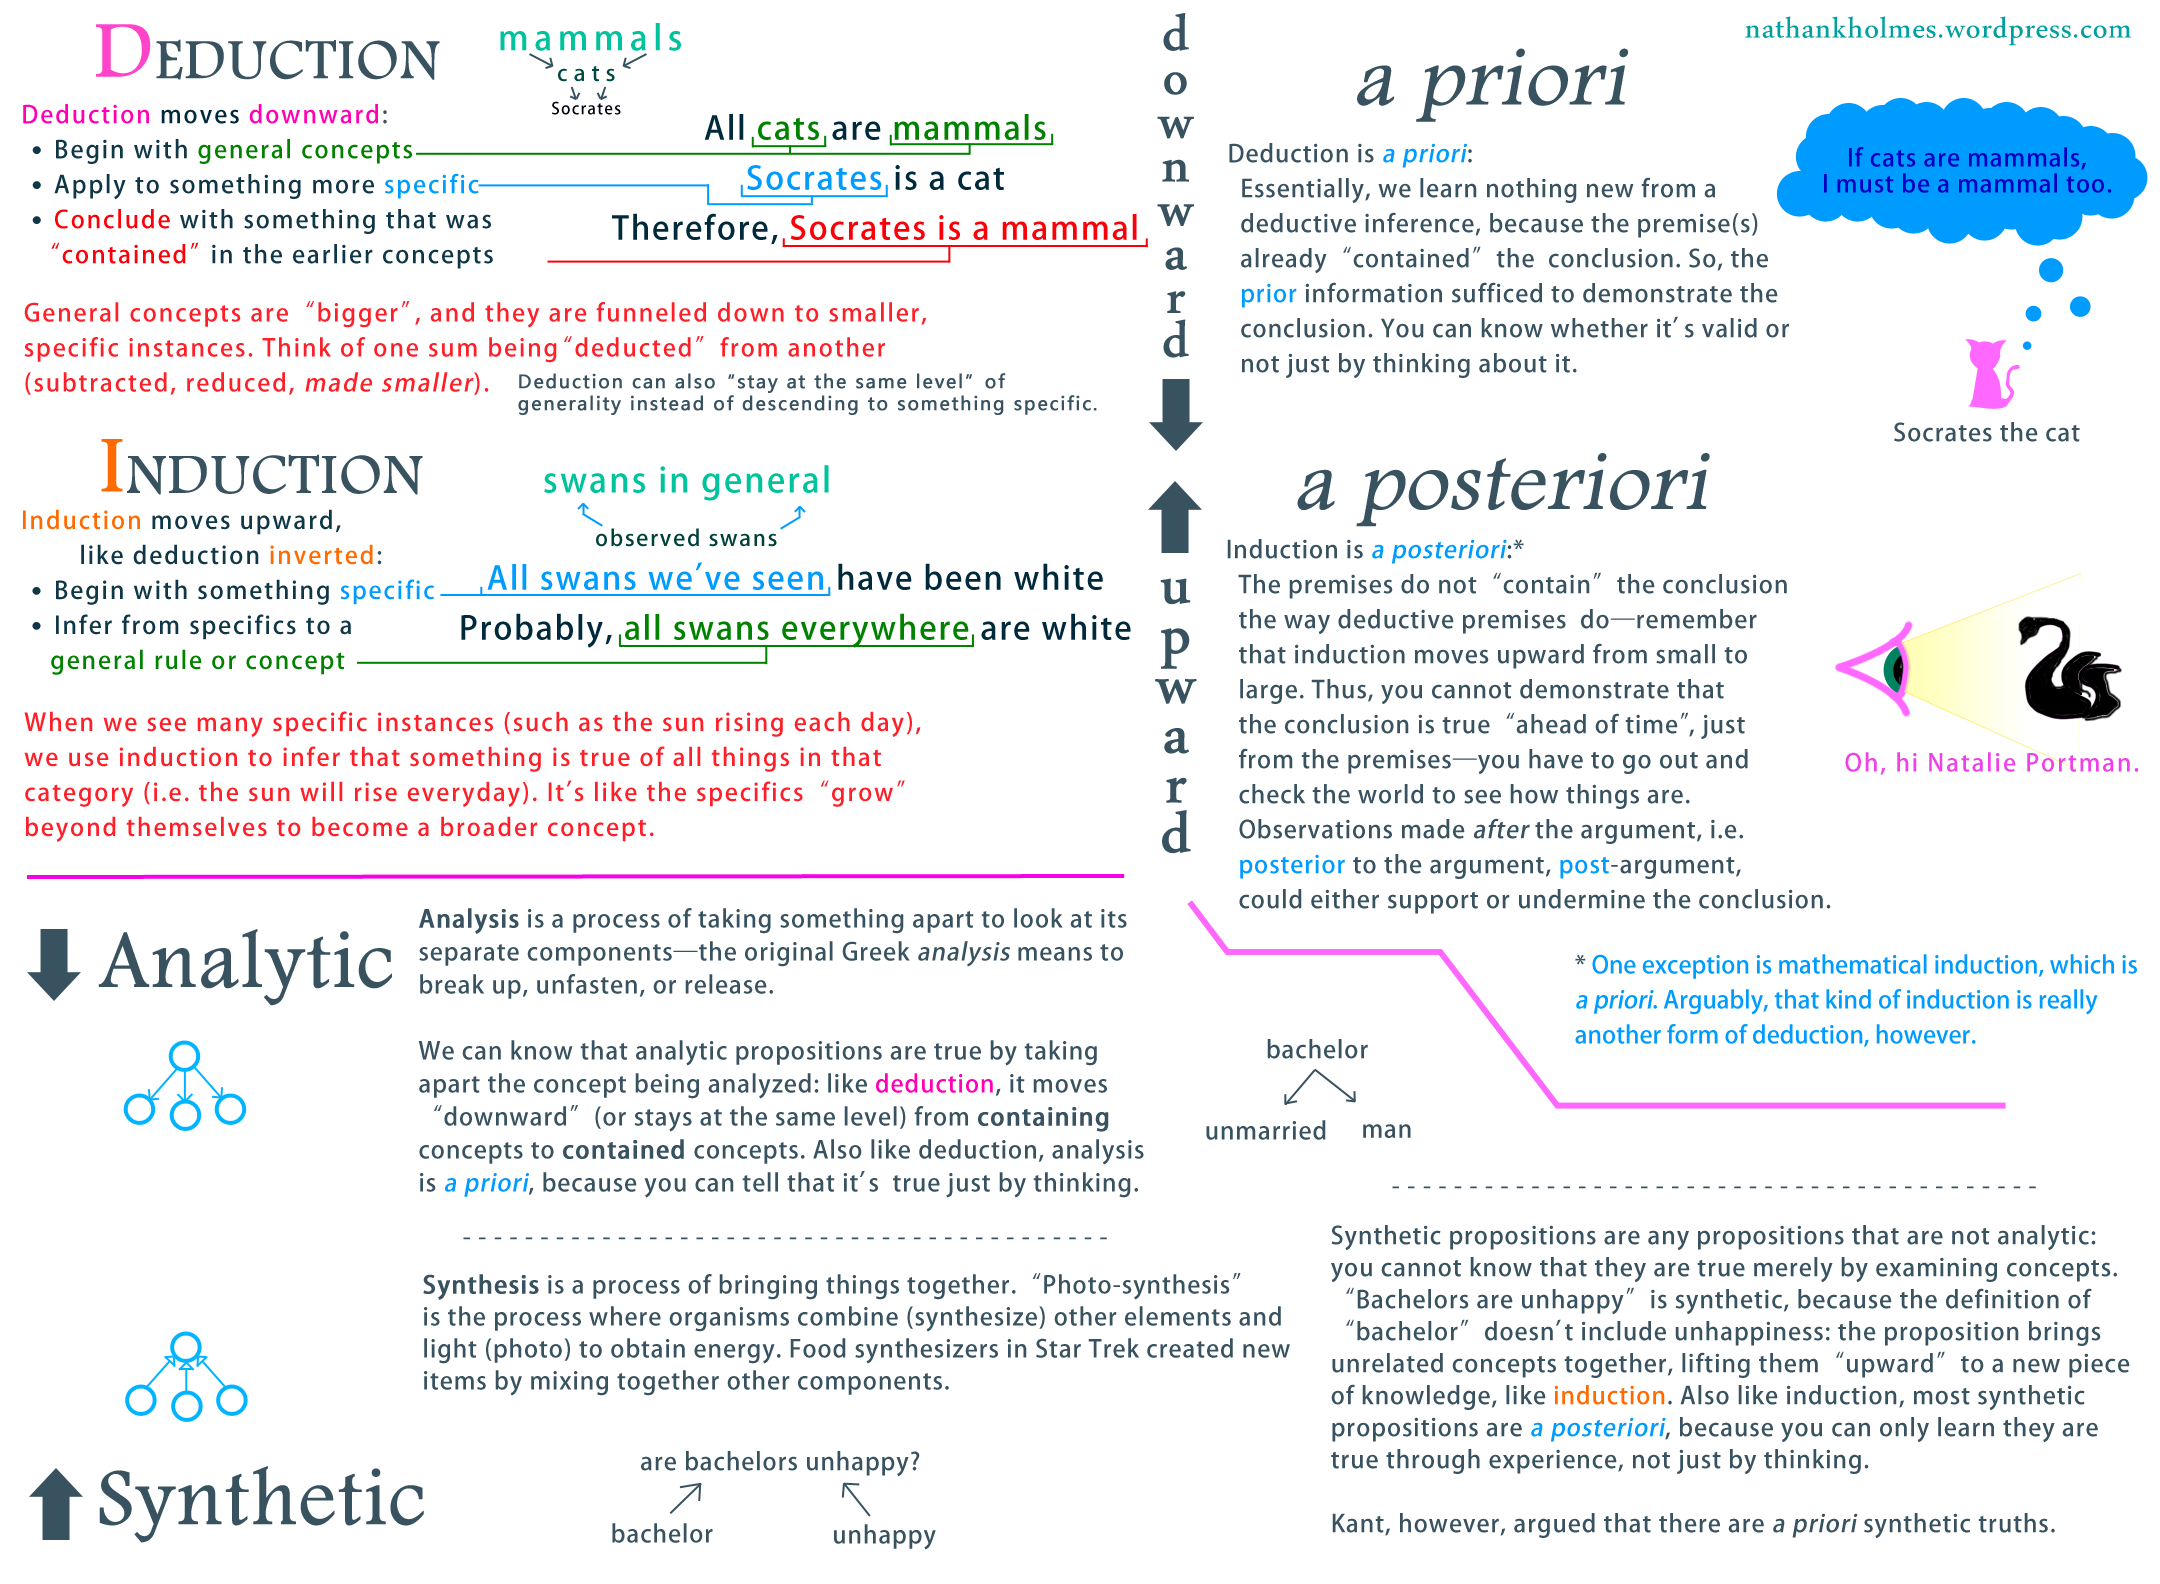
\includegraphics[scale=0.14]{./nathanholmes.png}
  \end{figure}
\end{frame}

\begin{frame}
  \frametitle{Brownian Motion}
  \begin{description}
  \item[Immanuel Kant] Many solutions that Kant presents for philosophical
  puzzles depend on his idea that there are synthetic a priori truths:
  truths that do not follow from the rules of language but can be
  recognized without reference to experience. Examples are
  the reliability of induction (solving Hume's problem of induction),
  mathematical truths, and (yes, that's embarrassing) the Euclidean
  nature of space.
  \end{description}
\end{frame}

\begin{frame}
  \frametitle{Brownian Motion}
  \begin{description}
  \item[Willard Van Orman Quine] Quine wrote a passionate and
    influential paper about Carnap's analytic/synthetic distinction,
    inspiring naturalists (the philosophical kind) such as Penelope
    Maddy.
  \end{description}
In philosophy, if you are a naturalist, you believe that reality is
exhausted by nature (there aren't any real things that are not
natural) and the way to find things out about real things is to use
scientific method.
\end{frame}

\begin{frame}
  \frametitle{iClicker Question}
Choose from the following options. This item will be graded.
\begin{block}{iClicker Question}
What does Foucault identify as a problem with modern discourse about sex?
\end{block}
\begin{description}
\item[A\hspace{.2in}$\blacktriangleright$] modernity is too
  body-focused (instead of mind-focused) in its sexuality
\item[B\hspace{.2in}$\blacktriangleright$] we talk about sexual desire too much
  (the endless mill of speech)
\item[C\hspace{.2in}$\blacktriangleright$] we don't talk about sex
  enough (repressed sexual desire must be articulated)
\item[D\hspace{.2in}$\blacktriangleright$] men want sex, women want
  conversation (gender imbalance with respect to verbal and sexual
  intimacy)
\end{description}
\end{frame}

\begin{frame}
  \frametitle{iClicker Question}
Choose from the following options. This item will be graded.
\begin{block}{iClicker Question}
According to Foucault, modern discourse about sex is intimately linked to
\end{block}
\begin{description}
\item[A\hspace{.2in}$\blacktriangleright$] the economic and political problem of population
\item[B\hspace{.2in}$\blacktriangleright$] the fear of sexually-transmitted disease
\item[C\hspace{.2in}$\blacktriangleright$] an erosion of monogamy due to homosexuality
\item[D\hspace{.2in}$\blacktriangleright$] the Christian dogma of the Trinity
\end{description}
\end{frame}

\end{document}
